% !TEX TS-program = pdflatex
% !TEX encoding = UTF-8 Unicode

% This is a simple template for a LaTeX document using the "article" class.
% See "book", "report", "letter" for other types of document.

\documentclass[11pt]{article} % use larger type; default would be 10pt
\usepackage{wrapfig}

\usepackage{float}
\usepackage[utf8]{inputenc} % set input encoding (not needed with XeLaTeX)
\usepackage[nonatbib]{nips_2016}
%%% Examples of Article customizations
% These packages are optional, depending whether you want the features they provide.
% See the LaTeX Companion or other references for full information.
\usepackage{natbib}
%%% PAGE DIMENSIONS
\usepackage{geometry} % to change the page dimensions
\geometry{a4paper} % or letterpaper (US) or a5paper or....
% \geometry{margin=2in} % for example, change the margins to 2 inches all round
% \geometry{landscape} % set up the page for landscape
%   read geometry.pdf for detailed page layout information

\usepackage{graphicx} % support the \includegraphics command and options

% \usepackage[parfill]{parskip} % Activate to begin paragraphs with an empty line rather than an indent

%%% PACKAGES
\usepackage{booktabs} % for much better looking tables
\usepackage{array} % for better arrays (eg matrices) in maths
\usepackage{paralist} % very flexible & customisable lists (eg. enumerate/itemize, etc.)
\usepackage{verbatim} % adds environment for commenting out blocks of text & for better verbatim
\usepackage{subfig} % make it possible to include more than one captioned figure/table in a single float
% These packages are all incorporated in the memoir class to one degree or another...

%%% HEADERS & FOOTERS
\usepackage{fancyhdr} % This should be set AFTER setting up the page geometry
\pagestyle{fancy} % options: empty , plain , fancy
\renewcommand{\headrulewidth}{0pt} % customise the layout...
\lhead{}\chead{}\rhead{}
\lfoot{}\cfoot{\thepage}\rfoot{}
\usepackage{graphicx}
\graphicspath{ {images/} }
\usepackage[]{algorithm2e}
\SetKwInOut{Parameter}{parameter}

%%% SECTION TITLE APPEARANCE
\usepackage{sectsty}
\allsectionsfont{\sffamily\mdseries\upshape} % (See the fntguide.pdf for font help)
% (This matches ConTeXt defaults)

%%% ToC (table of contents) APPEARANCE
\usepackage[nottoc,notlof,notlot]{tocbibind} % Put the bibliography in the ToC
\usepackage[titles,subfigure]{tocloft} % Alter the style of the Table of Contents
\renewcommand{\cftsecfont}{\rmfamily\mdseries\upshape}
\renewcommand{\cftsecpagefont}{\rmfamily\mdseries\upshape} % No bold!

%%% END Article customizations

%%% The "real" document content comes below...

\title{Player Modelling Using NMF In Recommender Systems And Classification Problems}
\author{
	Ronghao Yang \\
	School of Computer Science\\
	University of Waterloo\\
	Waterloo, ON, N2L 3G1 \\
	\texttt{r39yang@uwaterloo.ca}
}

\begin{document}
\maketitle

\begin{abstract}
Player modelling methods are commonly seen in video games. Such methods are implemented to improve players' sanctification and user experience. Other than being popular in video games, player modelling methods can also be used for recommender systems  and classification problems. Users are being modelled by such methods so that a corresponding item can be recommended/classified to the user based on his/her user type.

\end{abstract}
\section{Introduction}
Have you ever wondered, why can't you find the best music on Spotify? Or the most interesting book on Amazon? Or the finest hotel in the city of New York? In today's world, we want the service we get from the service providers (no matter online or offline) to be tailored to our interests, which means the services these days better to be personalized to amaze the customers. This is why recommendation systems are crucial in such business applications.\\
At some point, we can also view some of the recommendation problems as classification problems. Recommending a corresponding item to a user is no different from clustering this user into a item group. For example, the dataset we are going to work on for this project is a hotel recommendation problem, recommending a hotel to a user is clustering this user into a hotel cluster.\\
In the paper, I am going to introduce one of the player modelling methods called non-negative matrix factorization to tackle the problems, and analyse the performance of the method together with its disadvantages, moreover, explore its potential use in different fields. 
\section{Non-negative Matrix Factorization (NMF)}\label{introduction}
\paragraph{• Introduction to NMF}\mbox{}\\
$NMF$ is a matrix factorization algorithm which factorizes a big matrix $V$($m$ by $n$) into two smaller matrices $W$($m$ by $r$) and $H$($r$ by $n$).
\begin{equation}\label{eq1}
V\approx W \times H
\end{equation}
For each column $v_{i}$ in $V$, we have
\begin{equation}
v_{i} \approx W \times h_{i}
\end{equation}
where $h_{i}$ is the corresponding $i$th column in $H$, in other words, every column in $V$ is a linear combination of $W$, where $H$ is the coefficient matrix.\\
Geometrically, $NMF$ projects the data points in a higher dimensional space to a lower dimensional space formed by the basis vectors in $W$, and $H$ contains the projected coefficients.\\
To integrate the theory with the context, matrices are commonly seen in recommendation problems, with columns and rows being users and the corresponding items. When $NMF$ factorizes such a matrix into $W$ and $H$, the columns in $W$ contains the hidden features of the original matrix. Each basis vector in $W$ can be viewed as basic user type, every user therefore is represented as a linear combination of such basic user types which are.
\begin{equation}
u = a_1w_1+a_2w_2+....+a_rw_r
\end{equation}
where $u$ is a single user and $a_is$ are the coefficients.\\
Moreover, such user-item matrices are usually sparse (with high percentage of missing values), $NMF$ with EM algorithm can reconstruct the original matrix by filling out the missing values.
\paragraph{• Related work}\mbox{}\\
In 2014, Yu $\&$ Riedl from Georgia Tech have published a paper\cite{nmf1} about a recent success of $NMF$ for interactive narrative recommendation system. The goal of the research was to build a drama manager that learns a model of the player's storytelling preferences and automatically recommends a narrative experience that is predicted to optimize the player's experience while conforming to the human designer's storytelling intentions \cite[p.~1]{nmf1}.\\
In their research, a new method called $Prefix-Based\;Collaborative\;Filtering$ (PBCF) \cite[p.~2]{nmf1} has been introduced in which each prefix is a sequence of story plots. Based on $PBCF$, a prefix-rating matrix was constructed in which each row represents a prefix, each column represents a player, every entry in the matrix is the numerical rating rated by a player for a prefix. Similar to most recommendation problems, this matrix is sparse, due to the nature of the project that it is impossible for a single player to encounter all the prefixes and for a single prefix node to be encountered by all players.
\begin{figure}[H]
\caption{Prefix rating matrix $\cite[p.~4]{nmf1}$}
\centering
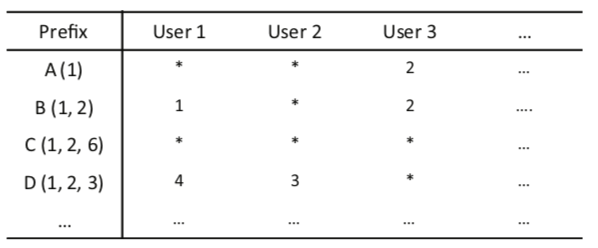
\includegraphics[width=0.5\textwidth]{prefixrating}
\end{figure}
The $NMF$ algorithm was applied to this matrix to learn the player types so that the prefix that has the highest rating is recommended to the reader. In their research, the prediction accuracy of option selection reached by $NMF$ at the experimental branching plot point is 76.26\% \citep[p.14]{nmf1}, which is the highest among all the collaborative filtering algorithms they have implemented.
\paragraph{• NMF update rule}\mbox{}\\
In $Algorithms\;for\;Non-negative\;Matrix\; Factorization$ published by Daniel F. Lee and H. Sebastian Seung in 2001, several $NMF$ updating rules have been introduced. One of which is
\begin{equation}
H_{\alpha\mu} = H_{\alpha\mu}\frac{(W^{T}V)_{\alpha\mu}}{(W^{T}WH)_{\alpha\mu}}, W_{i\alpha} = W_{i\alpha}\frac{(VH^{T})_{i\alpha}}{(WHH^{T})_{i\alpha}} \; \citep[p.~3]{nmfalg}
\end{equation}
This update rule guarantees the convergence of $NMF$. However, it does not deal with missing values in the dataset. To recover missing values in the dataset, we use EM algorithm. In the beginning of the update, we initialize the missing values in the matrix to be random. After each iteration of update, we set the corresponding entries in V to be the known values in the original dataset. We keep doing so until the error converges.
\section{Experiment}
\subsection{Dataset}
The dataset we use for experiment is the Expedia hotel recommendation dataset from Kaggle competition \cite{kaggle} in 2016. This dataset contains the hotel booking information of more than 2,000,000 users, of which the training set is obtained from 2013 and 2014 user data and the test set is obtained from 2015 user data.\\
In the data set, each column represent a user, each column contains a feature of the user. All of the feature variable are non-negative numerical variable except for date variable. For the purpose of simplifying of the data set, I have removed the date columns. Then the user types will only be represented by numerical values.\\
However, for privacy purposes, $Expedia$ has encoded many of the feature values, which makes the problem harder since the original values have changed. Moreover, some of the feature columns contain missing values. This might also create some challenge to the problem.
\subsection{User modelling and feature selection}
As has been said, when using $NMF$ for building the user model, each basis user type is represented by the combination of different features. For example, assume we have $W$ as a user model which has 4 columns ($w_{1}, w_{2}, w_{3}, w_{4}$). $w_{1}$ represent users who love luxurious hotels, $w_{2}$ represent users who prefer cheaper hotels, $w_{3}$ represent users who want to live in down-town, $w_{4}$ represent users who desire great hotel service. Then a new user maybe of 10\% of type 1, 30\% of type 2, 20\% of type 3 and 40\% of type 3.\\    
For feature selection, in some cases, we may also be able to select the number of basis based on some prior or domain knowledge. For example, mentioned in Yu \& Riedl's paper, the Interactive storytelling system PaSSAGE uses Robin’s Laws five game player schemes: Fighters, Power Gamers, Tacticians, Storytellers, and Method Actors. A player is modelled as a vector where each dimension is the strength of one of the type\citep[p.2]{nmf1}. However, in our case, no proven prior knowledge is available. $NMF$ is capable of selecting the number basis user type by running cross validations. The number of basis that generates the smallest cross validation error is selected.\\
The loss metric is set to the rmse (root-mean-square error) value between two matrices.
\begin{equation}
rmse_{A,B} = \sqrt{avg((A-B)^{2})}
\end{equation}
\paragraph{• Algorithm}\mbox{}\\
For this project, $KNN$ has been implemented as a complementary algorithm to $NMF$ for predicting the hotel clusters. Each user type is simply defined by the numerical features in the training set, such as search location, etc. Different from Yu \& Riedl's experiment, instead of using V from equation \ref{eq1} for prediction, we use H instead.\\
In the beginning of the training process, we apply $NMF$ on the training set to compute the user model $W_{train}$ and the user coefficients of the training set$H_{train}$ . Then we apply the computed model $W_{train}$ on the testing set to obtain the testing coefficients ($H_{test}$) of the testing users. Once we have the coefficients of testing users, we know what types of users they are. Then we go back to the training set and apply$KNN$ on $H_{train}$ and $H_{test}$ to find what hotel cluster users that have the similar coefficients choose, then we use that hotel cluster as a prediction for the unknown users. The algorithms are the following:\\
For computing the user coefficients, we use the same algorithm \cite[p.6]{nmf1} introduced in Yu and Ridel's paper. \\\\
\begin{algorithm}[H]
\SetKwData{Left}{left}
\SetKwData{This}{this}
\SetKwData{Up}{up}
\SetKwFunction{Union}{Union}
\SetKwFunction{FindCompress}{FindCompress}
\SetKwInOut{Input}{input}
\SetKwInOut{Output}{output}
\Input{User model $W_{train}$, Initial $R_{train}$ with missing values}
\Output{User coefficients H}
\BlankLine
\emph{Initialize H}\;
\While{not convergent }{
Compute R' using $R' = W\times H$\\
Set the corresponding number in $R'$ to be known values in $R_{train}$\\
Recompute H using $H_{\alpha\mu}$ = $H_{\alpha\mu}\frac{(W^{T}R)_{\alpha\mu}}{(W^{T}WH)_{\alpha\mu}}$
}
\caption{User Coefficients Prediction Algorithm}\label{H}
\end{algorithm}\mbox{}
Once we have the user coefficients of both training set and testing set, we apply KNN(K-nearest neighbours) on $H_{train}$ and $H_{test}$ for clustering.\\
\begin{algorithm}[H]
\SetKwData{Left}{left}
\SetKwData{This}{this}
\SetKwData{Up}{up}
\SetKwFunction{Union}{Union}
\SetKwFunction{FindCompress}{FindCompress}
\SetKwInOut{Input}{input}
\SetKwInOut{Output}{output}
\Input{User coefficients in training set $H_{train}$\\
 User coefficients in testing set $H_{test}$\\
 Clusters for training set $C_{train}$\\
 Number of clusters k}
\Output{Predicted clusters for testing set $C_{test}$}
\BlankLine
\ForEach{$h_{i}$ \textbf{in} $H_{test}$}{
Find k nearest points in $H_{train}$ using KNN\\
For these k nearest points, find the majority of their corresponding clusters in $C_{train}$\\
Set $c_{i}$ in $C_{test}$ to be that cluster
}
\caption{Cluster Prediction Using KNN}\label{KNN}
\end{algorithm}
\section{Results}
The two images below are the results for number of basis selection using cross validation. See from the figures below, with number of basis from 1 to 20, the lowest rmse is still as high as $10^{5}$.\\
\begin{figure}[H] 
  \begin{minipage}[H]{0.5\linewidth}\label{ m1cv1} 
    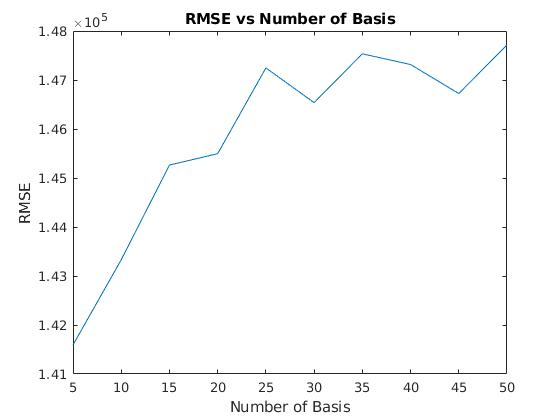
\includegraphics[width=1\linewidth]{m1CV1.jpg} 
    \caption{Cross validation with number of basis 5, 10, 15, .., 50} 
  \end{minipage} 
  \begin{minipage}[H]{0.5\linewidth}\label{ m1cv2} 
    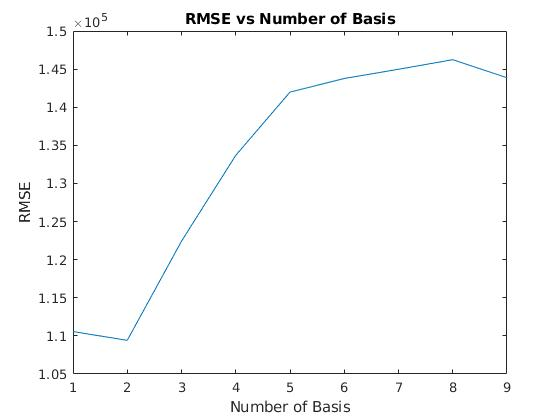
\includegraphics[width=1\linewidth]{m1CV2.jpg} 
    \caption{Cross validation with number of basis 1, 2, 3, ...9} 
  \end{minipage} 
  \hfill
\end{figure}\mbox{}\\
Although basis 2 has the lowest rmse value, this value is still way far away from a "good" (small) rmse value. Therefore, based on this observation, I do not expect for a good result from this method. To verify my expectation, I have tested multiple r's and k's (knn parameter) on the dataset. \\
The table below shows the accuracy of the first method, r is the number of basis in the user model, k is the knn parameter.

\centerline{
\begin{tabular}[H]{ |p{1.5cm}||p{1.5cm}|p{1.5cm}|p{1.5cm}|p{1.5cm}|p{1.5cm} | }
 \hline
 \multicolumn{6}{|c|}{Results} \\
 \hline
& r=2 &r=5&r=10&r=15&r=20\\
 \hline
k = 1   & 1.18\%    &1.20\% &   1.36\% &1.31\%&1.39\%\\
 \hline
k = 3  & 1.11\%    &1.17\%&   1.25\%&1.20\%&1.22\%\\
 \hline
 k = 5   & 1.14\%    &1.18\%&  1.24\%&1.28\%&1.24\%\\
 \hline
 k = 7  & 1.14\%    &1.29\%&   1.22\%&1.36\%&1.26\%\\
 \hline
 k = 9   & 1.19\%    &1.21\%&   1.29\%&1.25\%&1.34\%\\
 \hline
\end{tabular}
}\mbox{}\\
As we can see here, the results are disappointing as expected. There are 100 hotel clusters in the dataset, random guessing gives around 1$\%$ accuracy. The accuracy reached by $NMF$ algorithm is just slightly better than random guessing. This phenomenon might come from different factors. I will give a brief analysis of different factors in the later section.
\subsection{Comparison with other algorithms}
As in the papers and reports regarding the Expedia hotel recommendation competition, such player modelling methods have never been implemented. In one of the reports\citep{expedia1} from Indiana University, 6 different methods have been implemented, including naive bayes, decision trees, etc. The highest accuracy of their implementation is 52.36\% reached by Adaboost. However, among several different reports I have read, none of the them have mentioned how they dealt with missing values.
\section{Brief analysis of NMF}
Did our method really fail? Is using this method for recommendation/classification problem a bad idea?\\ 
To have deeper insights of $NMF$ and analyse what factors may affect the performance of $NMF$, I did several experiments. For the following experiments, I have set up a method to visualize the affecting factors. Let $V$ be an image, with or without missing values in it. Recall from section \ref{introduction}, we factorize $V$ into $W$ and $H$.
 \begin{equation}\label{eq3}
V\approx W \times H
\end{equation}
After factorization, we let $V'$ = $W \times H$. Then we compare the visualization of $V$ and $V'$.\
\begin{figure}[H] 
\centering
  \begin{minipage}[H]{0.32\linewidth}\label{ m1cv1} 
    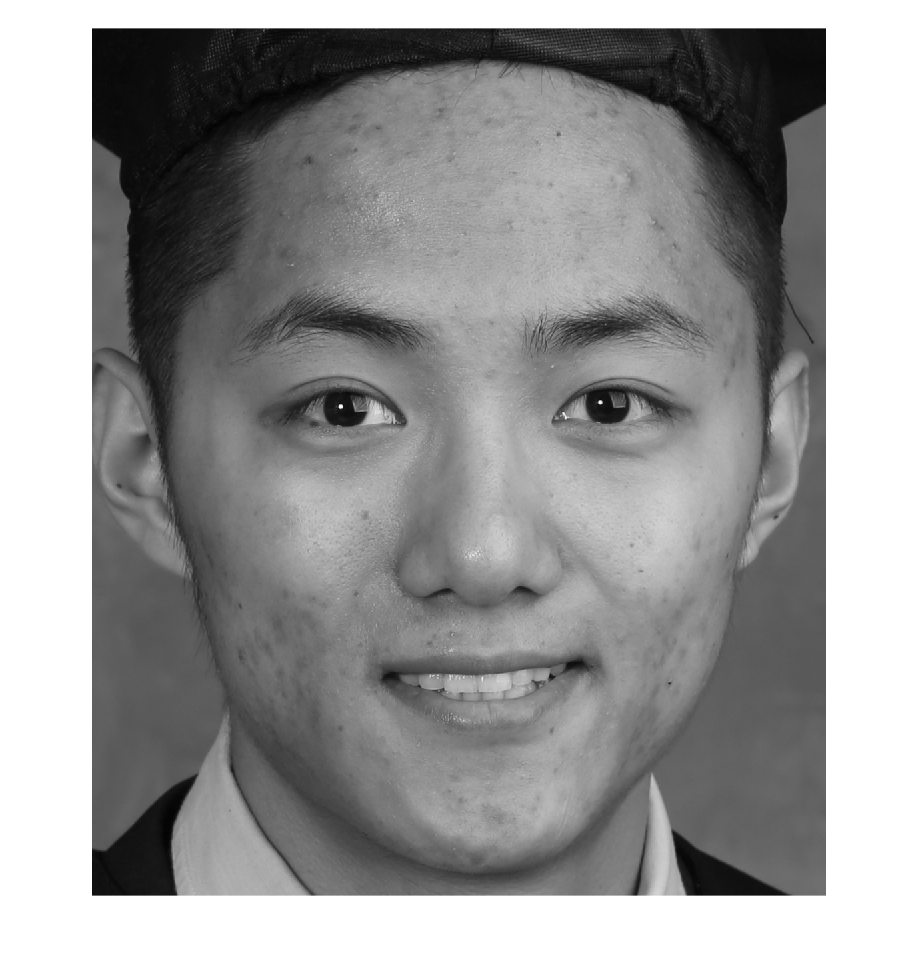
\includegraphics[width=\linewidth]{mySelfieOriginal.png} 
    \centering
    \caption{Original Image (Visualization of V)} 
  \end{minipage} 
\end{figure}
The original image has dimension 1300 by 1100, with 0\% missing values.
\subparagraph{• Percentage of Missing Values}\mbox{}\\
For the purpose of demonstration, I have set the number of basis in W to be 100 for the purpose of demonstration. Better selection of number of basis maybe available.
\begin{figure}[H]
\minipage{0.32\textwidth}
  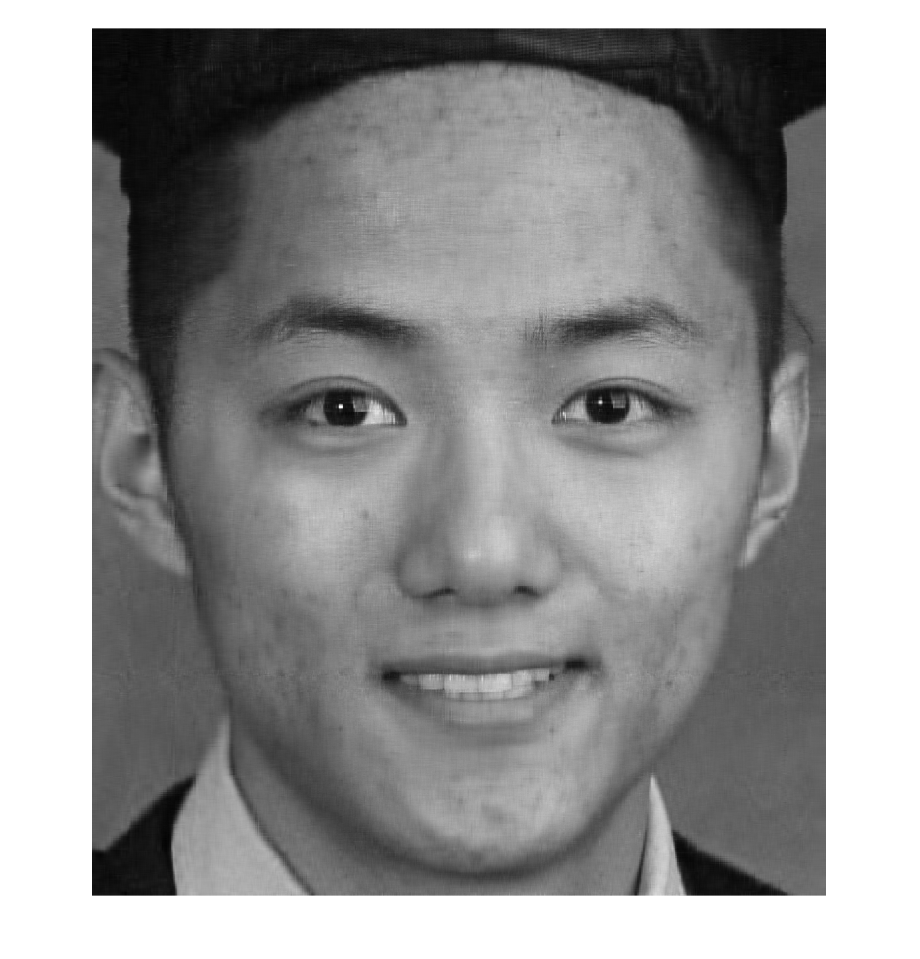
\includegraphics[width=\linewidth]{mySelfie50M100R.png}
  \caption{Reconstruction (V') of image with 50\% missing values in V}\label{fig:awesome_image1}
\endminipage\hfill
\minipage{0.32\textwidth}
  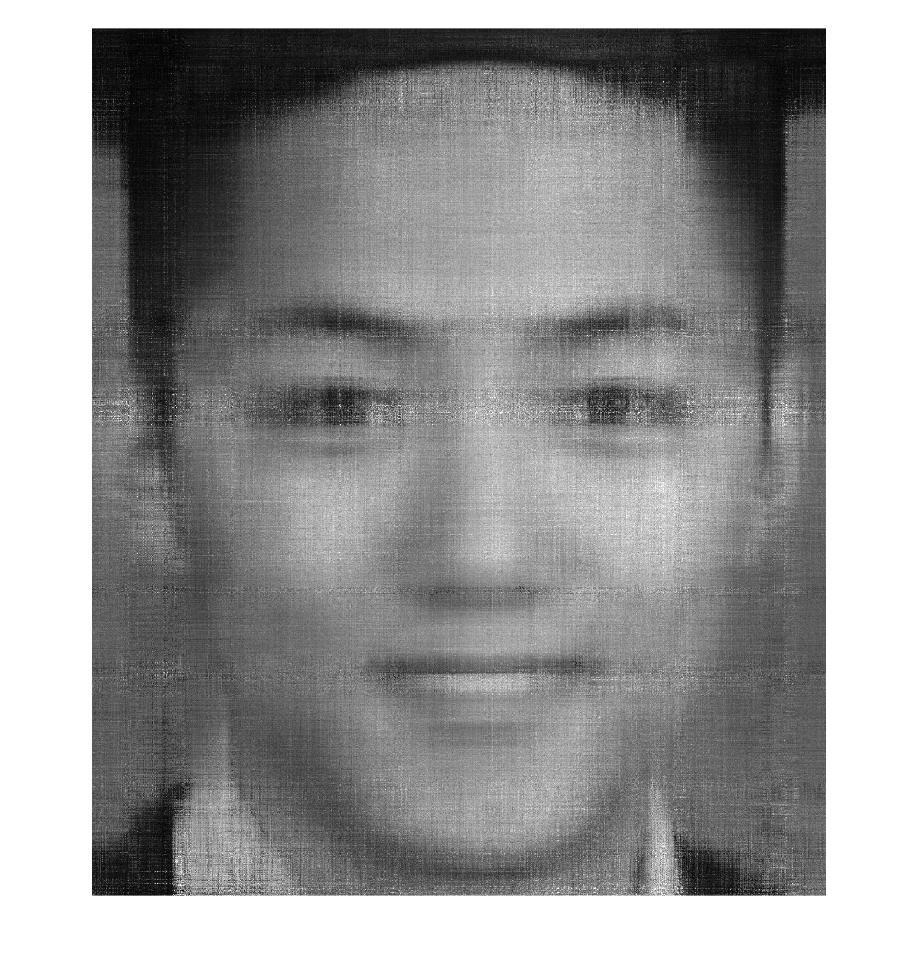
\includegraphics[width=\linewidth]{mySelfie90M100R.png}
  \caption{Reconstruction (V') of image with 90\% missing values in V}\label{fig:awesome_image2}
\endminipage\hfill
\minipage{0.32\textwidth}%
  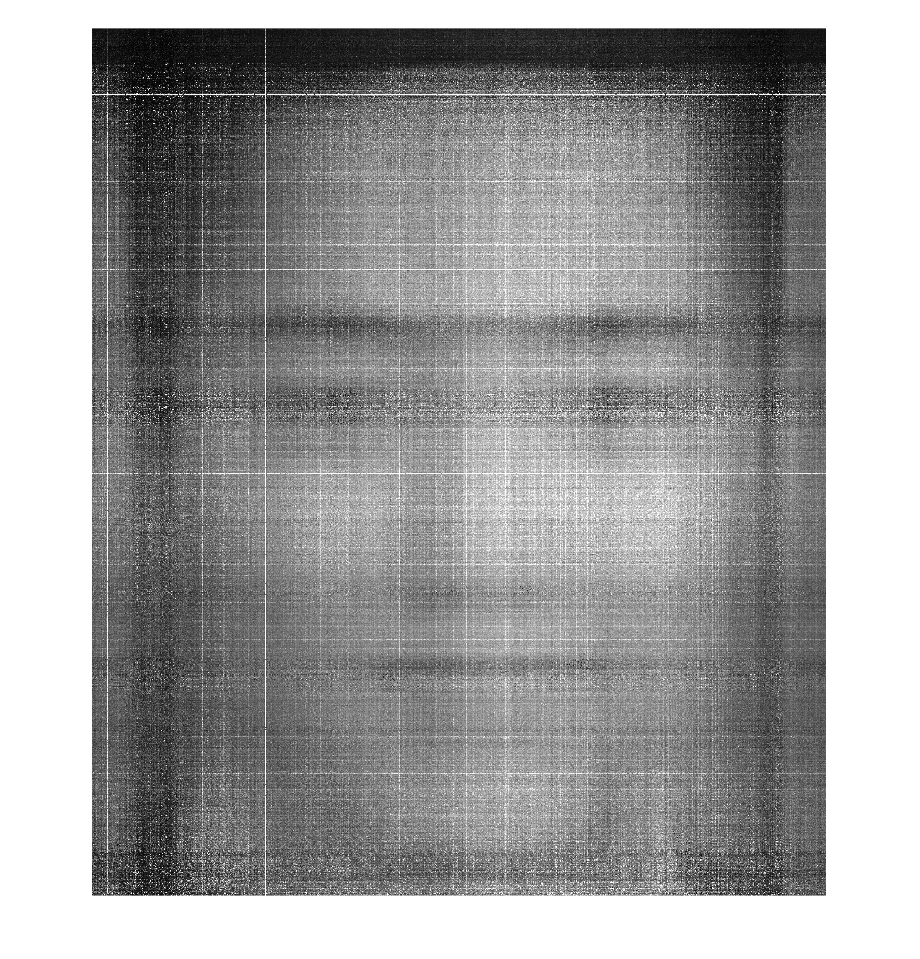
\includegraphics[width=\linewidth]{mySelfie95M100R.png}
  \caption{Reconstruction (V') of image with 95\% missing values in V}\label{fig:awesome_image3}
\endminipage
\end{figure}
As we can see here, the higher the percentage of missing values is, the worse the reconstruction is. However, this relationship does not appear to be linear. When the missing values go from 50\% to 90\%, we are still able to identify a face, however, when it goes from 90\% to 95\%, the face is merely identifiable.
\subparagraph{• Number of Basis}\mbox{}\\
For this subsection, I have set the percentage of missing values to be 50\%. We modify the number of basis in $W$, see how it affect the quality of the image reconstruction.
\begin{figure}[H]
\minipage{0.32\textwidth}
  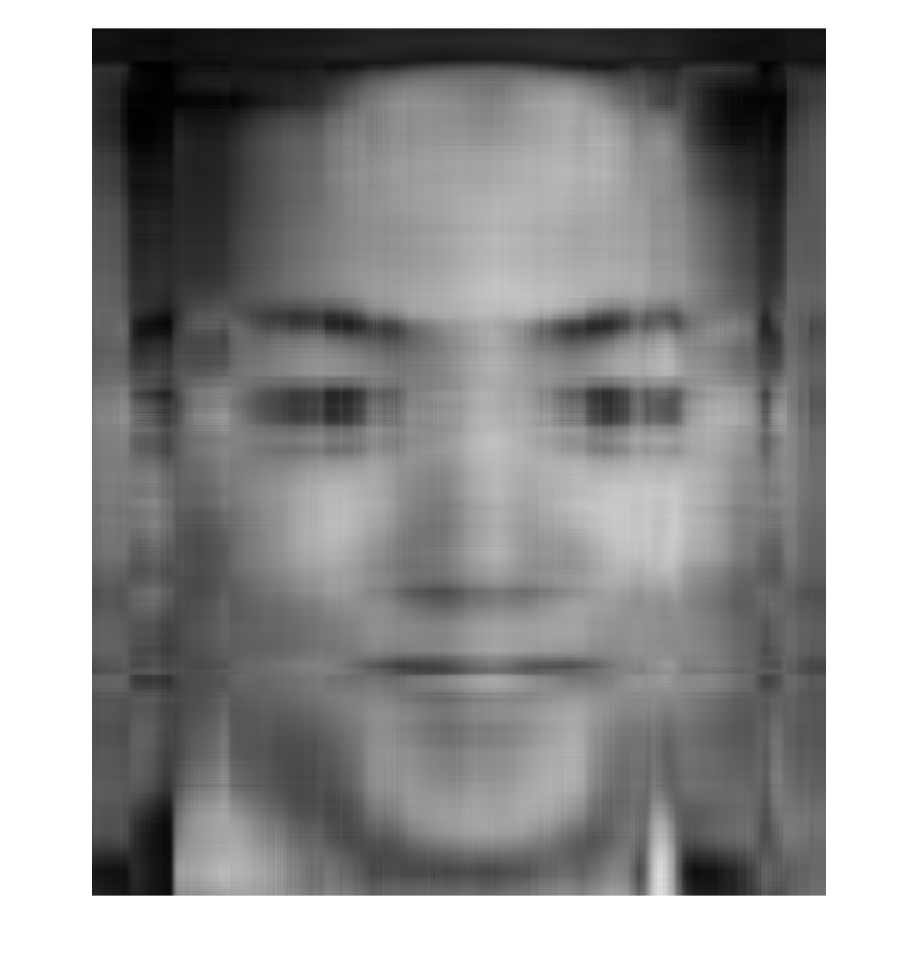
\includegraphics[width=\linewidth]{mySelfie50M5R.png}
  \caption{Reconstruction (V') of image with 5 basis in W}\label{fig:awesome_image1}
\endminipage\hfill
\minipage{0.32\textwidth}
  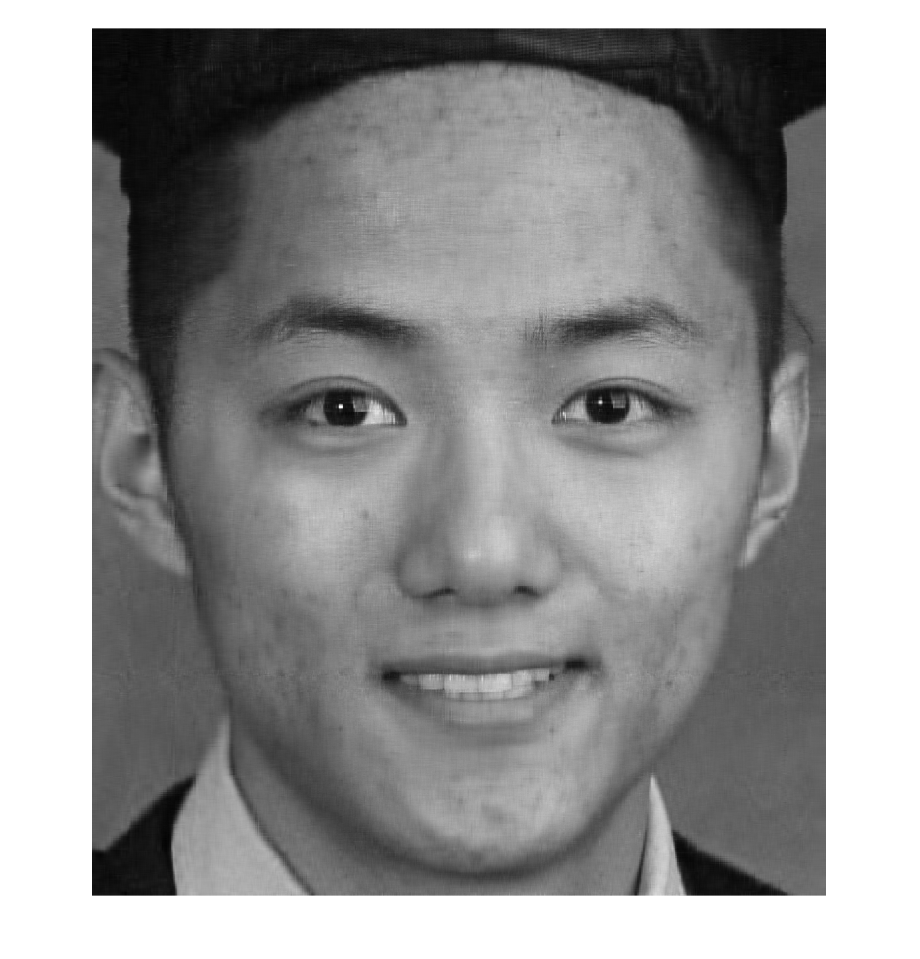
\includegraphics[width=\linewidth]{mySelfie50M100R.png}
  \caption{Reconstruction (V') of image with 100 basis in W}\label{fig:awesome_image2}
\endminipage\hfill
\minipage{0.32\textwidth}%
  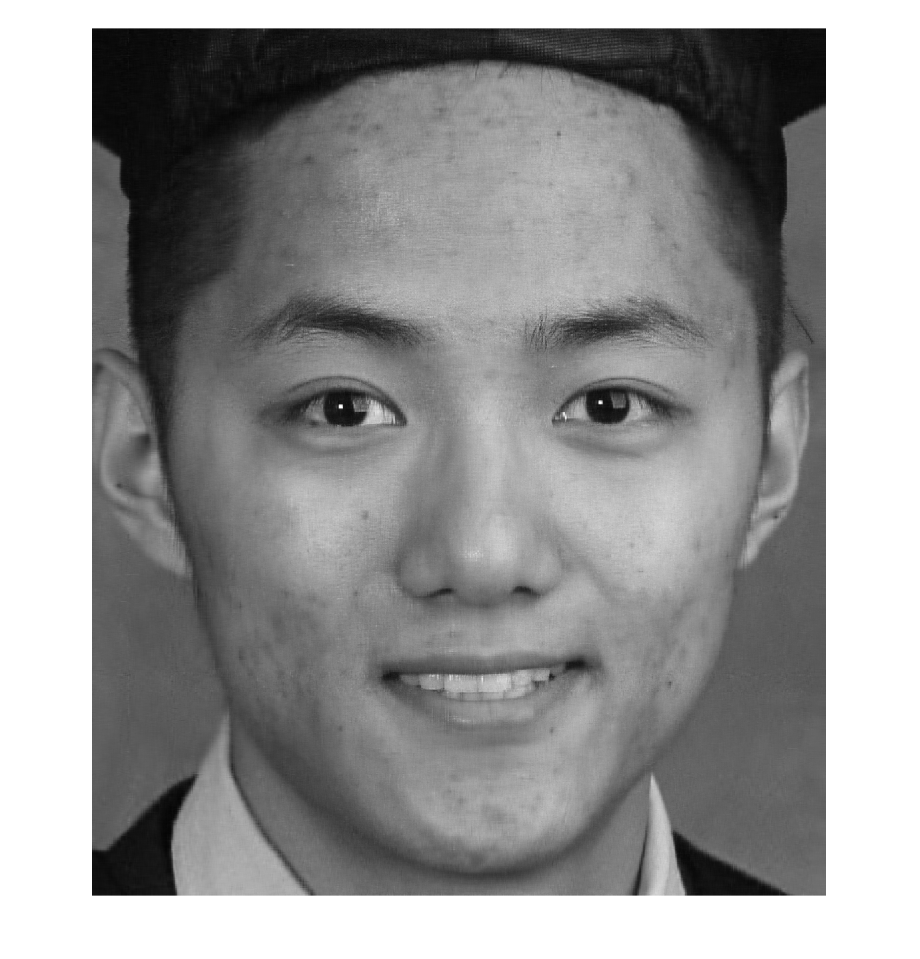
\includegraphics[width=\linewidth]{mySelfie50M200R.png}
  \caption{Reconstruction (V') of image with 200 basis in W}\label{fig:awesome_image3}
\endminipage
\end{figure}
When selecting the number of basis, we expect the number of basis to be the rank of V, since it is the smallest number of vectors that represent the vector space. However, in many cases, when we have missing values in V, rank is not defined. In such cases, we use cross validation for selecting basis. Here we can see, with only 5 basis, we suffer a huge information loss when reconstructing the original image. However, in real life scenarios, overfitting will arise when we have "too" many basis, running cross validation is a good practice to avoid overfitting.
\subparagraph{• Size of The Matrix}\mbox{}\\
For this subsection, we modify the size of $V$, see how it affect the quality of the image reconstruction. However, using visualization might not be a good idea, since if we resize the picture, they may not contain the same parts of the face in different images. Instead, we are showing a graph of rmse VS the size of image. Here we fix the percentage of missing values to be 90\% and the number of basis to be 100.
\begin{figure}[H] 
\centering
  \begin{minipage}[H]{0.65\linewidth}\label{ m1cv1} 
    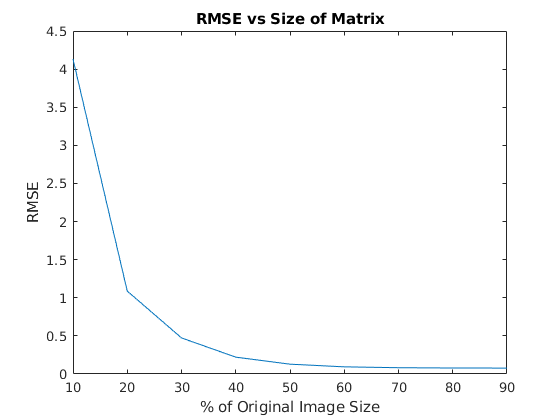
\includegraphics[width=\linewidth]{matrixSize.png} 
    \centering
    \caption{RMSE VS Matrix Size} 
  \end{minipage} 
\end{figure}
As we can see in the figure, RMSE drops substantially as the size of image increases from 10\% of the original image to 90\%. Moreover, the relationship between RMSE and the size of the matrix is not linear. For matrix $V$ of size 1300 by 1100 and with 90\% missing values. With 100 basis in $W$, rmse remains low as the size goes down to 50\% of it, therefore we should expect a good reconstruction even with 90\% missing values in such a small matrix. However, as the size of matrix keeps shirking, NMF just loses its mind. \\
As we have introduced earlier, NMF is a dimensionality reduction method which projects the data points from higher dimensional space to lower dimensional space. The value of the entries in the matrix are the information of the data points in different dimensions. The more missing values we have, the more information loss we suffer, $NMF$ will not be able to project well. With the same percentage of missing values, the bigger the matrix is, the more information we have left, with more information, $NMF$ performs better. In real life scenarios, one of the most straightforward ways to increase the size of the data matrix is to have more users. But how many is many? The answer should be as many as $NMF$ does not lose its mind. However, this might vary as the percentage of missing values, the number of basis, the nature of datasets differ.
\section{NMF on MNIST Dataset}
In the previous assignments, we have seen and used the MNIST dataset a few times. Many classification algorithms have shown great success on this dataset including KNN, CNN, etc. How my method will perform on this dataset? What if we have a huge percentage of missing values in the dataset, will this method still be able to classify correctly?\\
Note: For the following experiments, we assume the training set and the testing set come from the same distribution, therefore, we have the percentage of missing values in both training set and testing set to be the same. The number of basis and the knn parameters are selected by running 5-fold cross validation on the training set. Due to the time constraint, I have cut the training set from 60,000 images to 6,000 images.
\subsection{NMF \& KNN}
 In this section, we are going to test our algorithm on MNIST dataset and analyse the results. NMF is used for generating coefficient matrices $H_{train}$ and $H_{test}$. Then we apply KNN on $H_{train}$ and $H_{test}$ for clustering.\\\\
\centerline{
\begin{tabular}{ |p{3cm}|p{3cm}|  }
 \hline
 \multicolumn{2}{|c|}{Results} \\
 \hline
 Missing Value&Accuracy\\
 \hline
 30\%  &  95.4\%\\
 50\%& 94.1\%\\
 70\% &  86.9\%\\
 90\% &  52.1\%\\
  \hline
\end{tabular}
}
\subsection{NMF \& CNN}
In this section, instead of using $NMF$ and $KNN$ for clustering, we are going to apply a new method that uses CNN for clustering and $NMF$ for missing value recovery to analyse if $NMF$ is applicable in practice. The CNN net we used is VGG 11. For classification using CNN, we use $V_{train}$ and $V_{test}$ from equation \ref{eq1} instead of $H_{train}$ and $H_{test}$. $NMF$ here is used as a missing value recovering tool.\\\\
\centerline{
\begin{tabular}{ |p{3cm}|p{3cm}|  }
 \hline
 \multicolumn{2}{|c|}{Results} \\
 \hline
 Missing Value&Accuracy\\
 \hline
 30\%  &   98.69\%\\
 50\%& 96.77\%\\
 70\% &  92.36\%\\
 90\% &  52.87\%\\
  \hline
\end{tabular}
}\mbox{}\\\\
As we can see from above, even with a high percentage of missing values in both training set and testing set. After missing value recovery using NMF, CNN can still reach a high accuracy. 
\section{Discussion and future work}
As we have stated earlier in the introduction to NMF section, one of the most important assumptions of $NMF$ is linearity in the dataset, which assumes that a user can be represented as a linear combination of basis user types. However, it is not true in all cases, some datasets may not have linearity. Moreover, the performance is also largely affected by the percentage of missing values, the size of the data matrix, etc.\\
In 2006, the American entertainment company Netflix has hold a competition to call for researcher to come up with better solutions for their movie recommender system. The prize was 1 million dollars. The Netflix dataset contains 100 million anonymous movie ratings\cite{netflix}. In 2007, the Team Bellkor became the progress winner of the year. In their approach, NMF has been implemented as one of the methods to tackle the problem and has reached a relative good result (rmse = 0.8963) \citep[p.10]{netflix2007}. In addition to movie recommendation, this method has also shown great potential in document clustering and other applications.\\
For this project, I have combined NMF with KNN and CNN for both recommendation problem and classification problem. We have seen that NMF has shown great work in recovering missing values and clustering. Although NMF may fail on some datasets, for example, our Expedia hotel dataset, it has great potential in different sub-areas of both machine learning and artificial intelligence. In the future, the exploration of NMF on different datasets and different problems can be done to fully see the potential of this algorithm.\\

\section{Acknowledgement}
I gratefully acknowledge our instructor Dr.Yaoliang Yu for the amazing knowledge he shared with us and his support through out the term.

\bibliographystyle{plain}
\bibliography{report.bib}


\end{document}
